\linespread{1.5}
%use \usepackage{float}
\textbf{Solução}

\textbf{a)}
\begin{figure}[H]
    \centering
    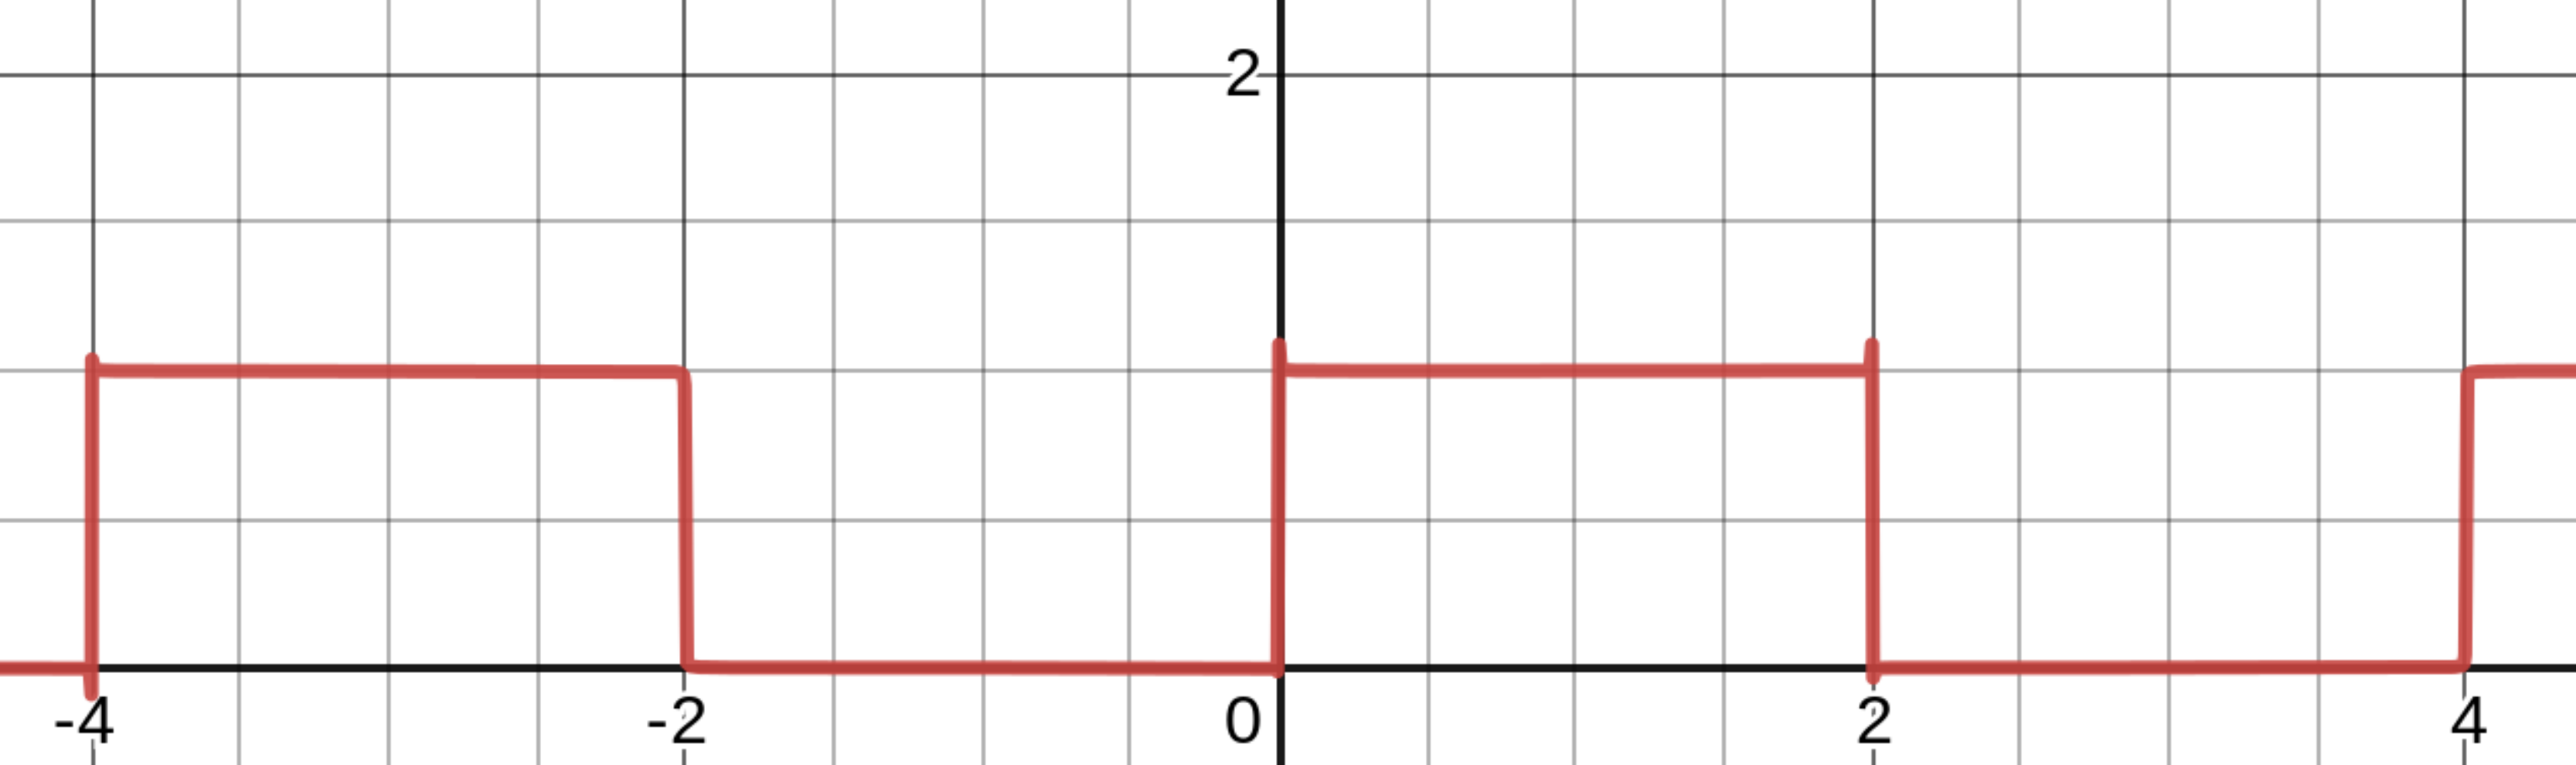
\includegraphics[width = 0.7\linewidth]{fig/sf13.png}
    \caption{Feita pelo site \textit{https://www.desmos.com/calculator} foi necessário limitar a série, o que permite ver os efeitos causados pela aproximação da série. Além disso no seu desenho deve mostrar os pontos que pertencem ou não aquela parte do gráfico, por exemplo: $x=4$ não pertence a $y=0$, mas sim a $y=1$, e assim sucessivamente. Além disso deve mostrar q os saltos de $y=0$ até $y=1$, não pertencem a função em si.
    }
\end{figure}

\textbf{b)}

Para determinar a série de Fourier real:
\begin{equation}
    \label{eq:Fourierserie}
    f(t) = a_0 + \sum_{k=1}^\infty a_k\cos{(kwt)} + b_k\sin{(kwt)}
\end{equation}

Precisamos determinar os seguintes coeficientes:
\begin{equation}
    \label{eq:a0Fourier}
    a_0 = \frac{1}{T}\int_0^T f(x)dx
\end{equation}
\begin{equation}
    \label{eq:akFourier}
    a_k = \frac{2}{T}\int_0^T f(x)\cos{(kwx)}dx
\end{equation}
\begin{equation}
    \label{eq:bkFourier}
    b_k = \frac{2}{T}\int_0^T f(x)\sin{(kwx)}dx
\end{equation}

Sabemos pelo comportamento da função que $T=4$, logo $w=\frac{\pi}{2}$.

Começando pelo $a_0$:

\begin{equation*}
    a_0 = \frac{1}{4}\left[\int_{-2}^0 0dt + \int^2_0 dt \right] = \frac{1}{4} \left[t\right]^2_0 \Rightarrow \boxed{a_0 = \frac{1}{2}}
\end{equation*}

Definimos então $a_k$:
\begin{equation*}
    a_k = \frac{2}{4}\left[\int^2_0 cos(kwt)\right] = \frac{1}{2}\left[\frac{sin(kwt)}{kw}\right]^2_0 = \frac{1}{2}sin\left(\frac{2\pi t}{2}\right) = \frac{sin(k\pi)}{2} 
\end{equation*}
Como sabemos que $\forall k \in \N$ $sin(k\pi) = 0$, portanto $\boxed{a_k = 0}$. Resolvemos então $b_k$:
\begin{equation*}
    b_k = \frac{2}{4}\left[\int^2_0 sin(kwt)dt\right] = \frac{1}{2}\left[\frac{-cos(kwt)}{kw}\right]^2_0 = \frac{1}{k\pi}\left(-cos\left(\frac{2k\pi}{2}\right)+cos(0)\right)
\end{equation*}
Sabemos que $cos(k\pi)=(-1)^k\forall k \in \N$, logo:
\begin{equation*}
   b_k = \frac{1-(-1)^k}{k\pi}
\end{equation*}
Se $k$ é par, $b_k = 0$, mas se $k$ é ímpar, então:
\begin{equation*}
    \boxed{b_k = \frac{2}{\pi(2k-1)}}
\end{equation*}
\begin{equation*}
    \boxed{\therefore f(t) = \frac{1}{2} + \sum^\infty_{k=1} \frac{2}{\pi(2k-1)}sin\left(\frac{(2k-1)\pi t}{2}\right)} 
\end{equation*}

\textbf{c)}

Quando $t=-2$, ou $t=2$ nos encontramos nas descontinuidades do gráfico. Portanto, nesses pontos temos que:
\begin{equation*}
    \lim_{t\rightarrow{}descont.} f(t) = \frac{f(t_-) + f(t_+)}{2}
\end{equation*}
\begin{enumerate}[i]
    \item t=-2
    \begin{equation*}
        \lim_{t\rightarrow-2} f(t) = \frac{f(t_-) + f(t_+)}{2} = \frac{1+0}{2} = \frac{1}{2} \rightarrow f(-2) = \frac{1}{2}
    \end{equation*}
    \item t=2
    \begin{equation*}
        \lim_{t\rightarrow2} f(t) = \frac{f(t_-) + f(t_+)}{2} = \frac{1+0}{2} = \frac{1}{2} \rightarrow f(2) = \frac{1}{2}
    \end{equation*}

Quanto ao caso $t=1$, temos pelo gráfico que como $f(t) = 1 $ para $t \in [0,2[$, temos que com $k\rightarrow\infty$, $f(t=1)=1$.
\end{enumerate}

\textbf{d)}
Com a série de Fourier complexa sendo dada por:
\begin{equation}
    \label{eq:Fouriercomplexa}
    f(x) = \sum^{+\infty}_{k=-\infty} c_k e^{ikwx}
\end{equation}
onde $c_k$ é dado por:
\begin{equation}
    \label{eq:ckFouerier}
    c_k = \frac{1}{T} \int^T_0 f(x)e^{-ikwx}dx
\end{equation}
teremos que:
\begin{equation*}
    c_k = \frac{1}{4}\int_{-2}^2 f(t)e^{\frac{-ikt\pi}{2}}dt = \frac{1}{4}\int_0^2e^{\frac{-ikt\pi}{2}}dt=\frac{1}{4}\frac{2}{-ik\pi}\left[e^{\frac{-ikt\pi}{2}}\right]^2_0 = \frac{-1}{2ik\pi}\left[e^{-ik\pi} - e^0 \right]
\end{equation*}
Sabemos que $e^{-ik\pi} = (-1)^k$, logo:
\begin{equation*}
    = \frac{i[(-1)^k-1]}{2k\pi}
\end{equation*}
o que nos da que para qualquer $k$ par $c_k=0$, já para $k$ ímpar:
\begin{equation*}
    \boxed{c_k =\frac{i}{\pi(2k-1)}} 
\end{equation*}
E assim:
\begin{equation*}
    \boxed{f(t) = \frac{i}{\pi}\sum^\infty_{-\infty} \frac{e^{\frac{ik\pi t}{2}}}{(2k-1)}}
\end{equation*}

\textbf{d)}

Sabendo que a relação entre os coeficientes de Fourier na forma complexa e na forma real é dado por:
\begin{equation*}
    \begin{cases}
    a_0 = c_0\\
    a_k = (c_k + c_{-k})\hspace{0.3cm}para\hspace{0.3cm}k\in\N\\
    b_k = i(c_k - c_{-k})\hspace{0.3cm}para\hspace{0.3cm}k\in\N
    \end{cases}
\end{equation*}
como $a_k = 0$ temos que $c_k = c_{-k}$ e portanto $b_k = i(c_k - c_{-k}) = 2ic_k$
\begin{equation*}
    \therefore c_k = \frac{b_k}{2i} = \frac{-ib_k}{2}
\end{equation*}
\begin{equation*}
    Sendo\hspace{0.3cm} b_k = \frac{2}{\pi(2k-1)}\Rightarrow \boxed{f(t) = \sum_{k=-\infty}^\infty \frac{-2ie^{\frac{i(2k-1)\pi t}{2}}}{2\pi(2k-1)}} 
\end{equation*}
